\chapter{\MakeUppercase{Metodologia e Processo de Desenvolvimento}}

Neste capítulo é descrito o processo de desenvolvimento adotado ao longo do estágio, abrangendo a aplicação da metodologia ágil \textit{Scrum}, o levantamento de requisitos e regras de negócio junto à empresa cliente e a arquitetura do \textit{front-end} construído. Para ilustrar as soluções tecnológicas, são apresentados, ao longo do texto, diagramas de alto nível e trechos simplificados do código desenvolvido, com a remoção de detalhes de estilo e de tratamento de erros para favorecer a legibilidade.

\section{Aplicação do \textit{Scrum} no Projeto}

O desenvolvimento da plataforma seguiu a metodologia \textit{Scrum}, organizada em \textit{Sprints} de duração fixa de duas semanas. No início de cada \textit{Sprint}, era realizada a reunião de \textit{planning}, na qual as tarefas priorizadas do \textit{Product Backlog} eram selecionadas e detalhadas no \textit{Sprint Backlog}. As tarefas eram acompanhadas em um quadro de tarefas dividido nas colunas de afazeres, em andamento, em revisão e concluído.

Para o gerenciamento do \textit{Product Backlog} e do \textit{Sprint Backlog} foi utilizado o \textit{Azure DevOps Boards}, ferramenta da \textit{Microsoft} voltada à gestão ágil de trabalho e ao acompanhamento de \textit{itens de trabalho} (\textit{Work Items}) ao longo do ciclo de desenvolvimento. Cada tarefa do \textit{backlog} possuía identificador, estado (por exemplo, \textit{New}, \textit{Approved} ou \textit{Committed}), título, área de produto e marcadores associados, o que facilitava a priorização e a distribuição das atividades entre os membros da equipe. A \autoref{fig:azure} apresenta um exemplo de tela do \textit{Azure DevOps Boards} com a listagem de \textit{Work Items} de um \textit{backlog}.

\begin{figure}[!htb]
\centering
\caption{Tela de \textit{backlog} do \textit{Azure DevOps Boards}.}
\label{fig:azure}
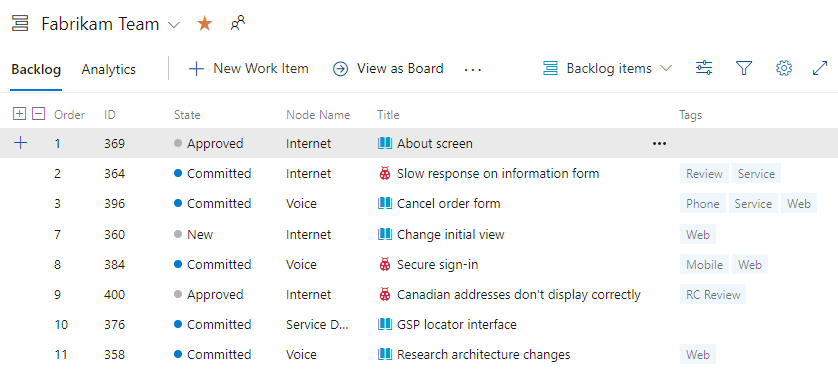
\includegraphics[width=0.95\textwidth,height=0.35\textheight,keepaspectratio]{imgs/azure_devops_backlog.png}
\fonte{Microsoft Learn. Disponível em: https://learn.microsoft.com/pt-br/azure/devops/boards/backlogs/create-your-backlog. Acesso em: maio 2026.}
\end{figure}

O acompanhamento diário ocorria por meio das \textit{daily meetings}, reuniões breves em que cada membro relatava o progresso, os planos do dia e eventuais impedimentos. Ao final de cada \textit{Sprint}, a \textit{Sprint Review} apresentava o incremento desenvolvido ao cliente, e a \textit{Sprint Retrospective} permitia à equipe refletir sobre o processo. A adoção desse fluxo possibilitou entregas incrementais à \novo{empresa cliente} e a validação contínua das funcionalidades, reduzindo o risco de retrabalho.

\section{Levantamento de Requisitos e Regras de Negócio}

O levantamento de requisitos foi conduzido de forma iterativa, em conjunto com a equipe da \novo{empresa cliente}. Como a empresa atua na pesquisa agrícola, muitas das regras de negócio eram específicas do domínio e não estavam formalmente documentadas, o que exigiu reuniões frequentes para esclarecer o comportamento esperado da plataforma.

\novop{O conjunto de regras que concentrou a maior complexidade foi o das regras de preenchimento dos protocolos, em que a obrigatoriedade e o formato de diversos campos dependiam do tipo de protocolo, da cultura selecionada e da classe do experimento. Como essas combinações não estavam descritas em nenhum documento, cada variação precisava ser esclarecida diretamente com a equipe do cliente antes de ser traduzida para o esquema de validação do formulário. Esses requisitos foram refinados a cada \textit{Sprint}, à medida que as telas eram apresentadas e validadas pelo cliente.}

\section{Arquitetura do \textit{Front-end} e Estrutura do Projeto}

A aplicação foi construída como uma \textit{Single Page Application} (SPA) em \textit{React} com \textit{TypeScript}, empacotada pelo \textit{Vite}. A organização do código seguiu uma separação por responsabilidades, distribuída em três camadas lógicas: a camada de apresentação, responsável pela renderização da interface; a camada de estado, responsável por manter os dados em memória durante a navegação; e a camada de acesso a dados, responsável pela comunicação com a API do servidor. A \autoref{fig:arquitetura} apresenta uma visão de alto nível dessa organização.

\begin{figure}[!htb]
\centering
\caption{Arquitetura em camadas do \textit{front-end} da plataforma de protocolos.}
\label{fig:arquitetura}
\vspace{0.3cm}

\begin{tikzpicture}[
  node distance=0.7cm,
  layer/.style={rectangle, draw, rounded corners, align=center,
                text width=11cm, minimum height=1.1cm, fill=gray!8},
  ext/.style={rectangle, draw, rounded corners, align=center,
              text width=7cm, minimum height=1cm, fill=gray!20},
  seta/.style={-{Latex}, thick}
]
\node[layer] (apres) {\textbf{Camada de Apresentação}\\ Componentes \textit{React}, \textit{Material UI}, \textit{TanStack Table} e \textit{ApexCharts}};
\node[layer, below=of apres] (estado) {\textbf{Camada de Estado}\\ \textit{Zustand} (estado global) e \textit{Formik} + \textit{Yup} (formulários)};
\node[layer, below=of estado] (dados) {\textbf{Camada de Acesso a Dados}\\ Camada de serviços sobre o \textit{Axios} (injeção de \textit{token} e \textit{refresh token}) e \textit{React Query} (\textit{cache} e sincronização)};
\node[ext, below=of dados] (api) {\textbf{API REST} (\textit{back-end})};
\draw[seta] (apres) -- (estado);
\draw[seta] (estado) -- (dados);
\draw[{Latex}-{Latex}, thick] (dados) -- (api);
\end{tikzpicture}

\vspace{0.2cm}
{\footnotesize Fonte: do autor (2026).}
\end{figure}

\novop{É importante destacar que o \textit{back-end} da plataforma, incluindo a API REST representada na \autoref{fig:arquitetura}, não foi desenvolvido pelo autor deste trabalho. Sua construção ficou a cargo de outra equipe da Zeeway, dedicada exclusivamente ao desenvolvimento do servidor, da modelagem do banco de dados e da implementação das regras de negócio do lado do servidor. Os capítulos seguintes detalham apenas as atividades realizadas na camada de \textit{front-end}.}

\novop{A coordenação entre as duas equipes foi baseada em uma estratégia de paralelização do trabalho a partir de uma interface comum. No início de cada nova funcionalidade, eram definidos em conjunto os contratos das chamadas à API, isto é, o caminho de cada \textit{endpoint}, o método HTTP utilizado e a estrutura dos dados de entrada e de saída. Com esse contrato acordado, as duas equipes passavam a trabalhar simultaneamente na mesma \textit{Sprint}: a equipe de \textit{back-end} implementava o \textit{endpoint} correspondente, enquanto a equipe de \textit{front-end} construía a tela e consumia inicialmente os dados em uma versão mascarada (\textit{mock}) que respeitava o contrato. Quando o \textit{endpoint} ficava disponível, a integração era feita substituindo a fonte dos dados pela API real. Ajustes pontuais no contrato eram negociados nas reuniões diárias ou na \textit{planning} da \textit{Sprint} seguinte, evitando que uma equipe ficasse permanentemente em ritmo diferente da outra.}

A estrutura de diretórios do projeto refletia essa separação de responsabilidades, agrupando os arquivos por função, conforme ilustrado no \autoref{cod:estrutura}. Os diretórios \texttt{components/}, \texttt{pages/} e \texttt{layouts/} concentram a parte visual da aplicação, enquanto \texttt{store/}, \texttt{services/} e \texttt{routes/} tratam, respectivamente, do estado global, da comunicação com a API e da definição das rotas. O diretório \texttt{hooks/} centraliza os \textit{hooks} customizados, como \texttt{useForm} e \texttt{useRoles}, e \texttt{utils/} reúne funções auxiliares reutilizadas em diferentes contextos.

\begin{lstlisting}[caption={Organização simplificada dos diretórios do projeto.}, label={cod:estrutura}, numbers=none]
src/
  components/   Componentes reutilizaveis (tabelas, modais, graficos)
  config/       Constantes e configuracoes globais
  contexts/     Contextos de React
  hooks/        Hooks customizados (useForm, useRoles, React Query)
  layouts/      Layouts de pagina (autenticacao e listagem)
  pages/        Telas (Login, Protocols, Dashboard, Clients, ...)
  routes/       Definicao e guarda de rotas
  services/     Camada de servicos e chamadas a API (Axios)
  store/        Estado global (Zustand)
  theme/        Tema do Material UI
  types/        Tipos TypeScript compartilhados
  utils/        Funcoes auxiliares (axios, arquivos, debounce)
\end{lstlisting}

Na camada de acesso a dados, todas as chamadas à API passavam por uma função de serviço (\texttt{httpRequest}) que anexava automaticamente o \textit{token} de acesso do usuário autenticado ao cabeçalho de autorização, evitando a repetição dessa lógica em cada requisição. Além disso, foi configurado um interceptador de resposta do \textit{Axios} responsável por renovar o \textit{token} de forma transparente sempre que a API retornava o código de erro 401, reenviando a requisição original com o novo \textit{token} obtido a partir do \textit{refresh token}. O \autoref{cod:interceptor} apresenta um trecho simplificado dessa configuração.

\begin{lstlisting}[caption={Trecho do interceptador de resposta para renovação do \textit{token} (\textit{refresh token}).}, label={cod:interceptor}]
axiosInstance.interceptors.response.use(
  (response) => response,
  async (error) => {
    const originalRequest = error.config;
    if (error.response?.status === 401 && !originalRequest._retry) {
      const { refreshToken } = loginStorePersist.getState().session;
      originalRequest._retry = true;
      const response = await axiosInstance.post("/user/refreshToken", {
        refreshToken,
      });
      const newToken = response.data.data.accessToken;
      loginStorePersist.getState().setLoginInfo({ data: response.data });
      originalRequest.headers["Authorization"] = `Bearer ${newToken}`;
      return axiosInstance(originalRequest);
    }
    return Promise.reject(error);
  }
);
\end{lstlisting}

O trecho registra um interceptador para todas as respostas do \textit{Axios}. A primeira função do par recebe as respostas bem-sucedidas e as devolve sem alteração. A segunda função trata os erros: ela inspeciona o código HTTP retornado e só age quando este é 401 (não autorizado) e quando a requisição original ainda não foi reexecutada, controle feito pela marcação \texttt{\_retry}. Nessa situação, o \textit{refresh token} é obtido do \textit{store} de autenticação e enviado em uma nova requisição ao \textit{endpoint} \texttt{/user/refreshToken}; quando essa requisição é bem-sucedida, o novo \textit{access token} é gravado no \textit{store} por meio de \texttt{setLoginInfo}, o cabeçalho de autorização da requisição original é atualizado e ela é reenviada de forma transparente para o usuário. Em qualquer outro caso, o erro é propagado normalmente.
